\section{Metodologia}

%-----------------------------------------------------%
\begin{frame}{Classificação da pesquisa}
\begin{itemize}
\item O objetivo de uma \textbf{pesquisa exploratória} é a familiarização com o assunto que ainda não foi bem explorado e existem poucas informações acerca do mesmo \cite{gil}.
\linebreak
\item A \textbf{pesquisa-ação} é um processo cíclico e contínuo, onde se planeja, implementa, descreve e avalia uma mudança para a melhoria de sua prática. Desta forma, há um aprendizado maior por parte do pesquisador durante o processo \cite{ramon}.
\end{itemize}
\end{frame}
%-----------------------------------------------------%
\begin{frame}{Planejamento da pesquisa}
\begin{itemize}
\item \href{run:./figuras/Processo_TCC.pdf}{Processo TCC}
\linebreak
\linebreak
\item \href{run:./figuras/scrum_adaptado.pdf}{Scrum adaptado para este TCC}
\end{itemize}

%  \begin{figure}[t]
%    \centering
%    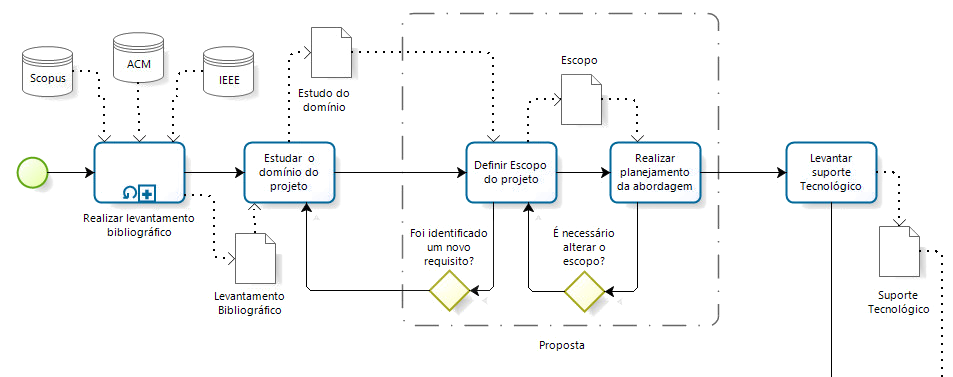
\includegraphics[height=\dimexpr10\textheight/14\relax]{figuras/processo1}
%    \caption{\href{run:./figuras/Processo_TCC.pdf}{Processo TCC (primeira parte)}}
%  \end{figure} 
\end{frame}
%-----------------------------------------------------%
%\begin{frame}{Planejamento da pesquisa II}
%  \begin{figure}[t]
%    \centering
%    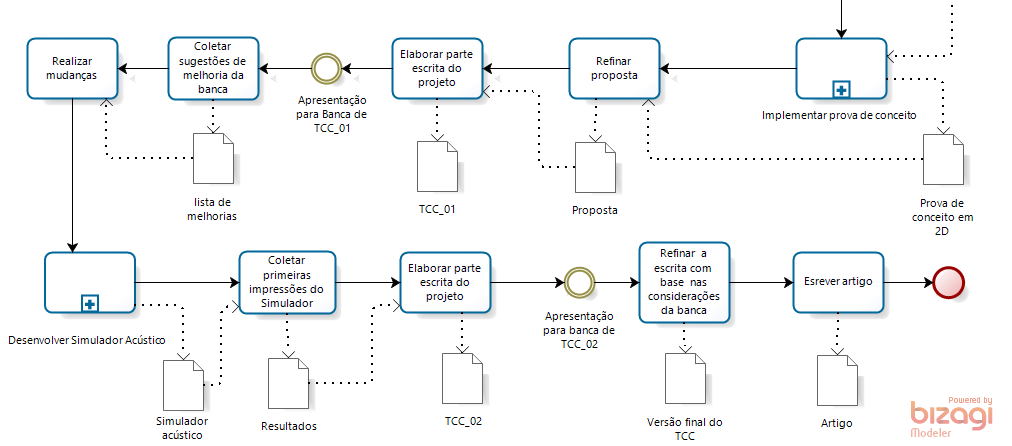
\includegraphics[height=\dimexpr10\textheight/14\relax]{figuras/processo2}
%    \caption{\href{run:./figuras/Processo_TCC.pdf}{Processo TCC (segunda parte)}}
%  \end{figure}
%\end{frame}
%-----------------------------------------------------%
\begin{frame}{Roadmap das sprints durante o desenvolvimento da ferramenta}
%  \begin{figure}[t]
%    \centering
%    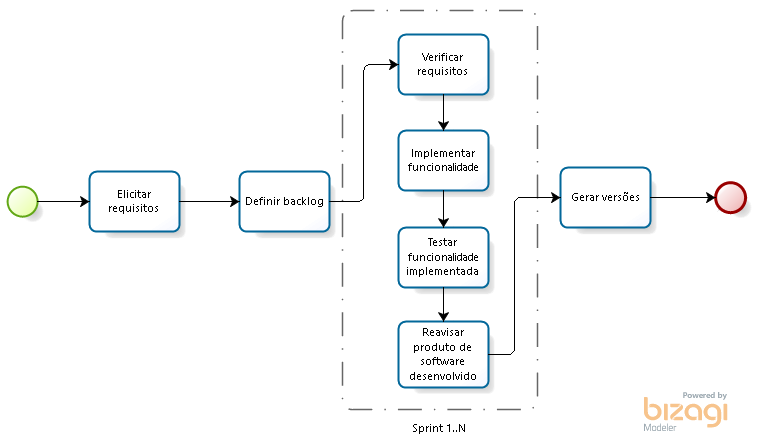
\includegraphics[height=\dimexpr10\textheight/14\relax]{figuras/Scrum}
%    \caption{\href{run:./figuras/scrum_adaptado.pdf}{Scrum adaptado para este TCC}}
%  \end{figure}
%\end{frame}
%-----------------------------------------------------%
%\begin{frame}{Metodologia adotada no desenvolvimento do simulador}

\begin{table}[]
\centering
\small
\caption{Roadmap}
\label{cronograma_sprints}
\begin{tabular}{|c|c|c|c|}
\hline
\textbf{Sprint}	& \textbf{Atividade} & \textbf{Data de início} & \textbf{Data de Término}	\\ \hline
Sprint 1  & Implementar US01 			& 07/06/2015     	& 14/06/2015      	\\ \hline
Sprint 2  & Implementar US02 			& 14/06/2015     	& 21/06/2015      	\\ \hline
Sprint 3  & Implementar US03 			& 21/06/2015     	& 28/07/2015      	\\ \hline
Sprint 4  & Implementar US10 			& 28/06/2015     	& 05/07/2015      	\\ \hline
Sprint 5  & Implementar US05 			& 05/07/2015     	& 12/07/2015      	\\ \hline
Sprint 6  & Implementar US04 			& 12/07/2015    	 	& 19/07/2015      	\\ \hline
Sprint 7  & Atividade de Refatoração		& 19/07/2015	 		& 26/07/2015	   		\\ \hline
Sprint 8  & Implementar US06 			& 26/07/2015     	& 02/08/2015      	\\ \hline
Sprint 9  & Implementar US11 			& 02/08/2015     	& 09/08/2015      	\\ \hline
Sprint 10 & Implementar US07 			& 09/08/2015     	& 16/08/2015      	\\ \hline
Sprint 11 & Implementar US08 			& 16/08/2015     	& 23/08/2015      	\\ \hline
Sprint 12 & Implementar US09 			& 23/08/2015     	& 30/08/2015      	\\ \hline
Sprint 13 & Atividade de Refatoração		& 30/08/2015     	& 06/09/2015	   		\\ \hline
\end{tabular}
\end{table}
\end{frame}
%-----------------------------------------------------%